\documentclass{standalone}
\usepackage{tikz}
\usetikzlibrary{patterns, positioning}
\usepackage[sfdefault]{ClearSans} %% option 'sfdefault' activates Clear Sans as the default text font
\usepackage[T1]{fontenc}

\begin{document}
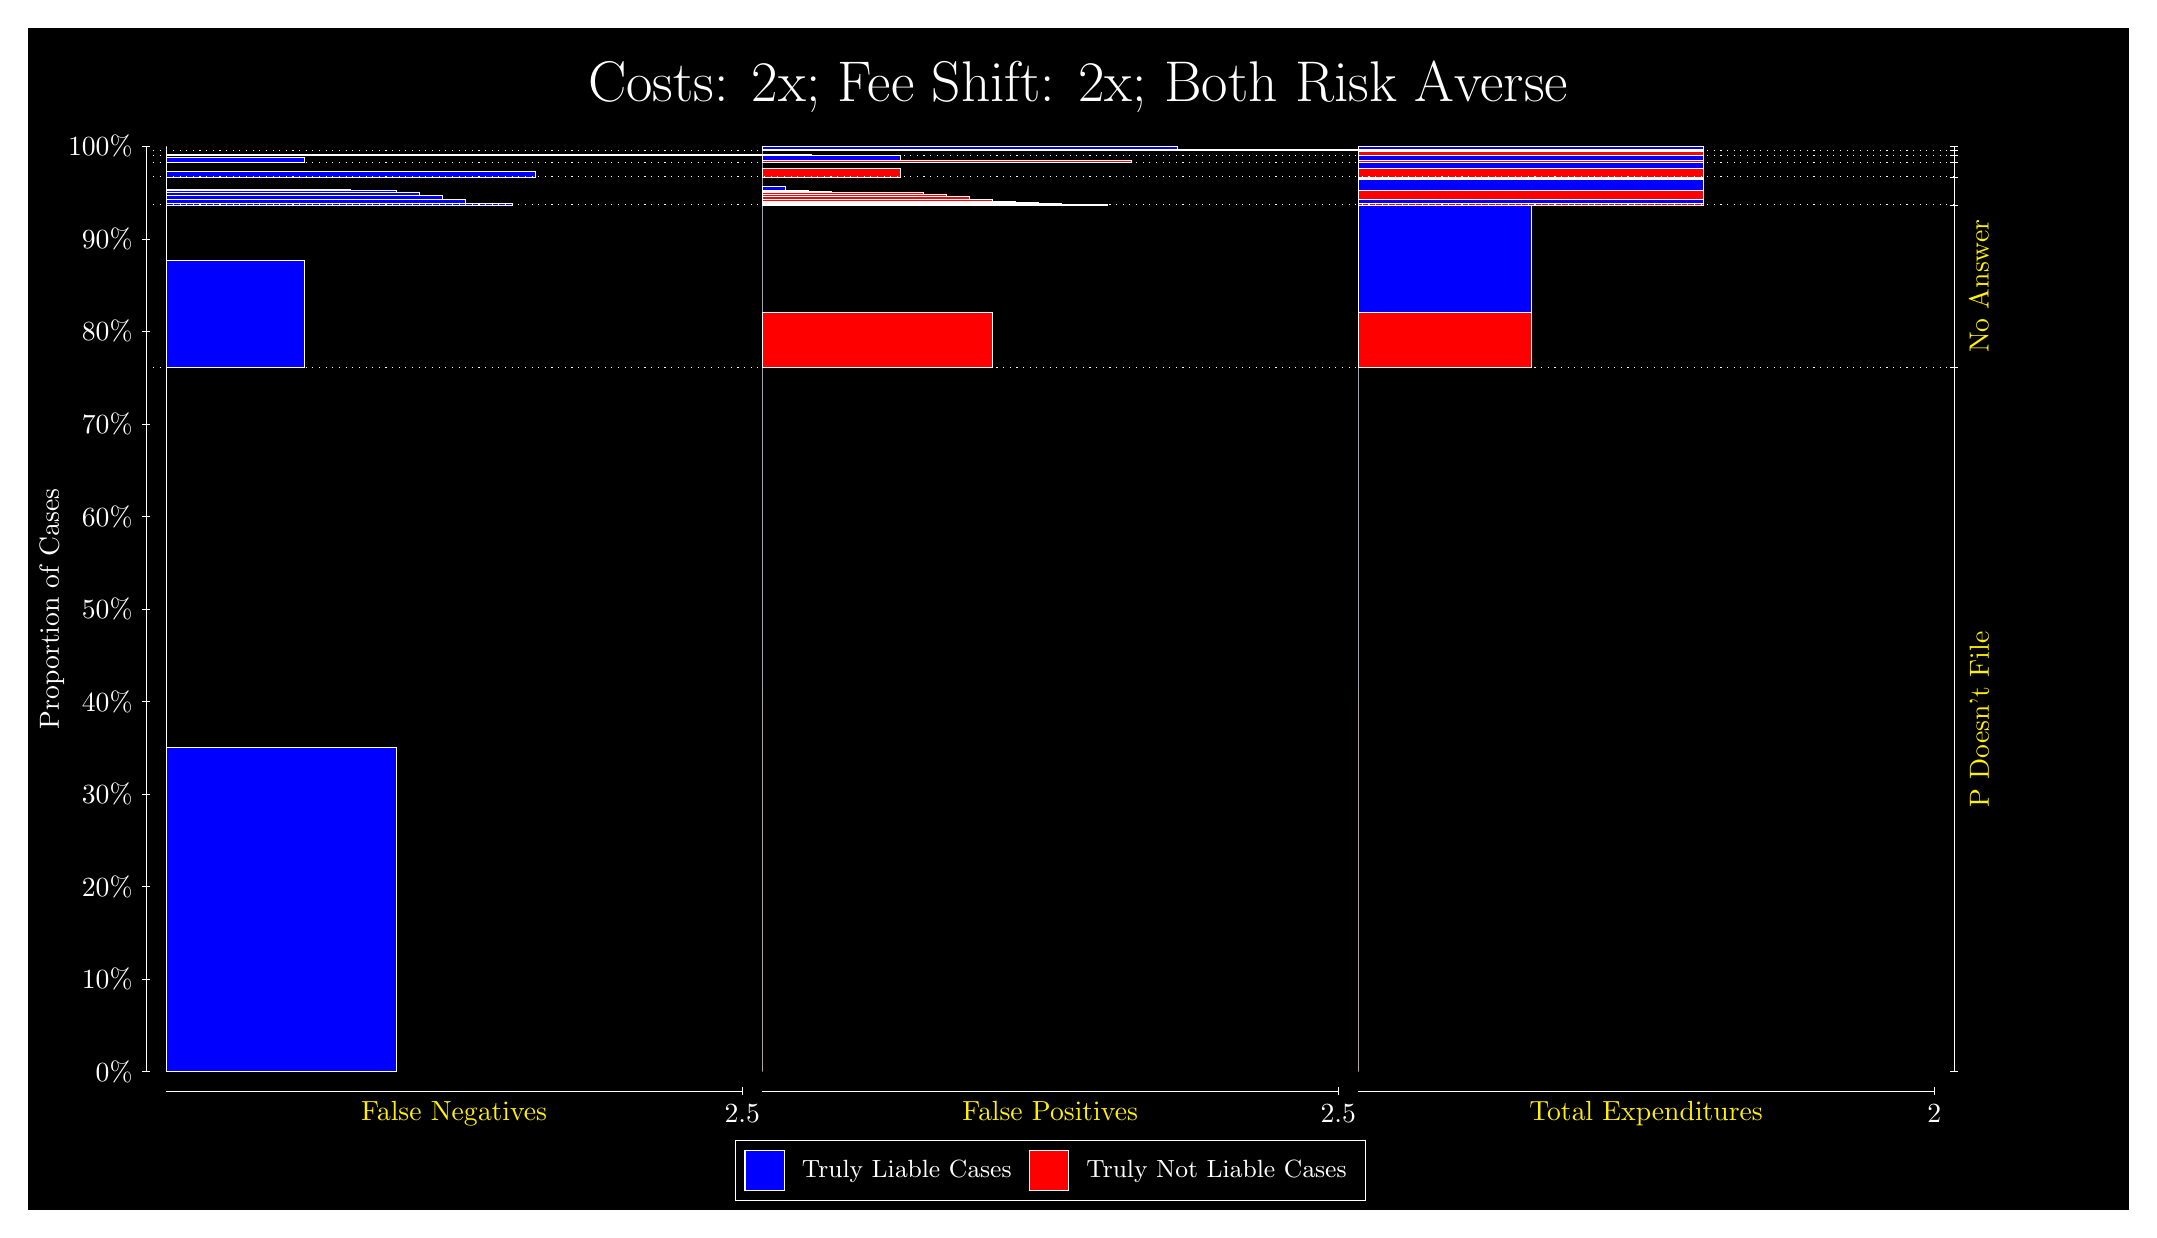
\begin{tikzpicture}
\draw[fill=black] (0,0) rectangle (26.667,15);
\draw[text=white] (0,13.5) rectangle (26.667,15) node[midway] {\huge Costs: 2x; Fee Shift: 2x; Both Risk Averse};
\draw[white, very thin] (1.5,1.75) -- (1.5,13.5);
\node[rotate=90, text=white, anchor=center] at (0.3, 7.625) {Proportion of Cases};
\draw[white, very thin] (1.45,1.75) -- (1.55,1.75);
\node[text=white, anchor=east] at (1.45, 1.75) {0\%};
\draw[white, very thin] (1.45,2.925) -- (1.55,2.925);
\node[text=white, anchor=east] at (1.45, 2.925) {10\%};
\draw[white, very thin] (1.45,4.1) -- (1.55,4.1);
\node[text=white, anchor=east] at (1.45, 4.1) {20\%};
\draw[white, very thin] (1.45,5.275) -- (1.55,5.275);
\node[text=white, anchor=east] at (1.45, 5.275) {30\%};
\draw[white, very thin] (1.45,6.45) -- (1.55,6.45);
\node[text=white, anchor=east] at (1.45, 6.45) {40\%};
\draw[white, very thin] (1.45,7.625) -- (1.55,7.625);
\node[text=white, anchor=east] at (1.45, 7.625) {50\%};
\draw[white, very thin] (1.45,8.8) -- (1.55,8.8);
\node[text=white, anchor=east] at (1.45, 8.8) {60\%};
\draw[white, very thin] (1.45,9.975) -- (1.55,9.975);
\node[text=white, anchor=east] at (1.45, 9.975) {70\%};
\draw[white, very thin] (1.45,11.15) -- (1.55,11.15);
\node[text=white, anchor=east] at (1.45, 11.15) {80\%};
\draw[white, very thin] (1.45,12.325) -- (1.55,12.325);
\node[text=white, anchor=east] at (1.45, 12.325) {90\%};
\draw[white, very thin] (1.45,13.5) -- (1.55,13.5);
\node[text=white, anchor=east] at (1.45, 13.5) {100\%};

\draw[white, very thin] (24.457,1.75) -- (24.457,13.5);
\draw[white, very thin] (24.407,1.75) -- (24.507,1.75);
\node[anchor=west] at (24.407, 1.75) {};
\draw[white, very thin] (24.407,10.69) -- (24.507,10.69);
\node[anchor=west] at (24.407, 10.69) {};
\draw[white, very thin] (24.407,12.757) -- (24.507,12.757);
\node[anchor=west] at (24.407, 12.757) {};
\draw[white, very thin] (24.407,13.113) -- (24.507,13.113);
\node[anchor=west] at (24.407, 13.113) {};
\draw[white, very thin] (24.407,13.292) -- (24.507,13.292);
\node[anchor=west] at (24.407, 13.292) {};
\draw[white, very thin] (24.407,13.389) -- (24.507,13.389);
\node[anchor=west] at (24.407, 13.389) {};
\draw[white, very thin] (24.407,13.45) -- (24.507,13.45);
\node[anchor=west] at (24.407, 13.45) {};
\draw[white, very thin] (24.407,13.5) -- (24.507,13.5);
\node[anchor=west] at (24.407, 13.5) {};

\draw[white, very thin, fill=blue] (1.75,1.75) rectangle (4.6775,5.873);
\draw[white, very thin, fill=red] (1.75,5.873) rectangle (1.75,10.69);
\draw[white, very thin, fill=blue] (1.75,10.69) rectangle (3.5065,12.055);
\draw[white, very thin, fill=red] (1.75,12.055) rectangle (1.75,12.757);
\draw[white, very thin, fill=blue] (1.75,12.757) rectangle (6.1413,12.775);
\draw[white, very thin, fill=blue] (1.75,12.775) rectangle (5.8486,12.782);
\draw[white, very thin, fill=blue] (1.75,12.782) rectangle (5.5558,12.823);
\draw[white, very thin, fill=blue] (1.75,12.823) rectangle (5.2631,12.875);
\draw[white, very thin, fill=blue] (1.75,12.875) rectangle (4.9703,12.922);
\draw[white, very thin, fill=blue] (1.75,12.922) rectangle (4.6775,12.937);
\draw[white, very thin, fill=blue] (1.75,12.937) rectangle (4.3848,12.948);
\draw[white, very thin, fill=blue] (1.75,12.948) rectangle (4.092,12.953);
\draw[white, very thin, fill=blue] (1.75,12.953) rectangle (3.7993,12.958);
\draw[white, very thin, fill=red] (1.75,12.958) rectangle (1.75,13.113);
\draw[white, very thin, fill=blue] (1.75,13.113) rectangle (6.4341,13.185);
\draw[white, very thin, fill=red] (1.75,13.185) rectangle (1.75,13.292);
\draw[white, very thin, fill=blue] (1.75,13.292) rectangle (3.5065,13.355);
\draw[white, very thin, fill=red] (1.75,13.355) rectangle (1.75,13.389);
\draw[white, very thin, fill=blue] (1.75,13.389) rectangle (9.9471,13.4);
\draw[white, very thin, fill=red] (1.75,13.4) rectangle (1.75,13.45);
\draw[white, very thin, fill=red] (1.75,13.45) rectangle (1.75,13.461);
\draw[white, very thin, fill=blue] (1.75,13.461) rectangle (1.75,13.5);
\draw[white, very thin, fill=red] (9.3189,1.75) rectangle (9.3189,6.5669);
\draw[white, very thin, fill=blue] (9.3189,6.5669) rectangle (9.3189,10.69);
\draw[white, very thin, fill=red] (9.3189,10.69) rectangle (12.246,11.391);
\draw[white, very thin, fill=blue] (9.3189,11.391) rectangle (9.3189,12.757);
\draw[white, very thin, fill=red] (9.3189,12.757) rectangle (13.71,12.761);
\draw[white, very thin, fill=red] (9.3189,12.761) rectangle (13.417,12.765);
\draw[white, very thin, fill=red] (9.3189,12.765) rectangle (13.125,12.773);
\draw[white, very thin, fill=red] (9.3189,12.773) rectangle (12.832,12.785);
\draw[white, very thin, fill=red] (9.3189,12.785) rectangle (12.539,12.806);
\draw[white, very thin, fill=red] (9.3189,12.806) rectangle (12.246,12.827);
\draw[white, very thin, fill=red] (9.3189,12.827) rectangle (11.954,12.868);
\draw[white, very thin, fill=red] (9.3189,12.868) rectangle (11.661,12.885);
\draw[white, very thin, fill=red] (9.3189,12.885) rectangle (11.368,12.911);
\draw[white, very thin, fill=blue] (9.3189,12.911) rectangle (10.783,12.916);
\draw[white, very thin, fill=blue] (9.3189,12.916) rectangle (10.49,12.922);
\draw[white, very thin, fill=blue] (9.3189,12.922) rectangle (10.197,12.933);
\draw[white, very thin, fill=blue] (9.3189,12.933) rectangle (9.9044,12.947);
\draw[white, very thin, fill=blue] (9.3189,12.947) rectangle (9.6116,12.995);
\draw[white, very thin, fill=blue] (9.3189,12.995) rectangle (9.3189,13.113);
\draw[white, very thin, fill=red] (9.3189,13.113) rectangle (11.075,13.22);
\draw[white, very thin, fill=blue] (9.3189,13.22) rectangle (9.3189,13.292);
\draw[white, very thin, fill=red] (9.3189,13.292) rectangle (14.003,13.326);
\draw[white, very thin, fill=blue] (9.3189,13.326) rectangle (11.075,13.389);
\draw[white, very thin, fill=red] (9.3189,13.389) rectangle (9.3189,13.439);
\draw[white, very thin, fill=blue] (9.3189,13.439) rectangle (9.3189,13.45);
\draw[white, very thin, fill=red] (9.3189,13.45) rectangle (17.516,13.461);
\draw[white, very thin, fill=blue] (9.3189,13.461) rectangle (14.588,13.5);
\draw[white, very thin, fill=red] (16.888,1.75) rectangle (16.888,6.5669);
\draw[white, very thin, fill=blue] (16.888,6.5669) rectangle (16.888,10.69);
\draw[white, very thin, fill=red] (16.888,10.69) rectangle (19.083,11.391);
\draw[white, very thin, fill=blue] (16.888,11.391) rectangle (19.083,12.757);
\draw[white, very thin, fill=red] (16.888,12.757) rectangle (21.279,12.778);
\draw[white, very thin, fill=blue] (16.888,12.778) rectangle (21.279,12.825);
\draw[white, very thin, fill=red] (16.888,12.825) rectangle (21.279,12.946);
\draw[white, very thin, fill=blue] (16.888,12.946) rectangle (21.279,13.084);
\draw[white, very thin, fill=red] (16.888,13.084) rectangle (21.279,13.096);
\draw[white, very thin, fill=blue] (16.888,13.096) rectangle (21.279,13.113);
\draw[white, very thin, fill=red] (16.888,13.113) rectangle (21.279,13.22);
\draw[white, very thin, fill=blue] (16.888,13.22) rectangle (21.279,13.292);
\draw[white, very thin, fill=red] (16.888,13.292) rectangle (21.279,13.326);
\draw[white, very thin, fill=blue] (16.888,13.326) rectangle (21.279,13.389);
\draw[white, very thin, fill=red] (16.888,13.389) rectangle (21.279,13.439);
\draw[white, very thin, fill=blue] (16.888,13.439) rectangle (21.279,13.45);
\draw[white, very thin, fill=red] (16.888,13.45) rectangle (21.279,13.461);
\draw[white, very thin, fill=blue] (16.888,13.461) rectangle (21.279,13.5);
\draw[white, dotted] (1.5,10.69) -- (24.457,10.69);
\draw[white, dotted] (1.5,12.757) -- (24.457,12.757);
\draw[white, dotted] (1.5,13.113) -- (24.457,13.113);
\draw[white, dotted] (1.5,13.292) -- (24.457,13.292);
\draw[white, dotted] (1.5,13.389) -- (24.457,13.389);
\draw[white, dotted] (1.5,13.45) -- (24.457,13.45);
\draw[white, very thin] (1.75,1.5) -- (9.0689,1.5);
\node[text=yellow, anchor=north] at (5.4094, 1.5) {False Negatives};
\draw[white, very thin] (9.0689,1.45) -- (9.0689,1.55);
\node[text=white, anchor=north] at (9.0689, 1.45) {2.5};

\draw[white, very thin] (9.3189,1.5) -- (16.638,1.5);
\node[text=yellow, anchor=north] at (12.978, 1.5) {False Positives};
\draw[white, very thin] (16.638,1.45) -- (16.638,1.55);
\node[text=white, anchor=north] at (16.638, 1.45) {2.5};

\draw[white, very thin] (16.888,1.5) -- (24.207,1.5);
\node[text=yellow, anchor=north] at (20.547, 1.5) {Total Expenditures};
\draw[white, very thin] (24.207,1.45) -- (24.207,1.55);
\node[text=white, anchor=north] at (24.207, 1.45) {2};

\node[text=yellow, centered, rotate=90] at (24.777, 6.2199) {P Doesn't File};
\node[text=yellow, centered, rotate=90] at (24.777, 11.723) {No Answer};






\draw (12.978300999999998,1.5) node[draw=none] (baseCoordinate) {};
\begin{scope}[align=center]
        \matrix[scale=0.5, draw=white, below=0.5cm of baseCoordinate, nodes={draw}, column sep=0.1cm]{
            \node[rectangle, draw, minimum width=0.5cm, minimum height=0.5cm, fill=blue] {}; &
            \node[draw=none, font=\small, text=white] (B) {Truly Liable Cases}; &
            \node[rectangle, draw, minimum width=0.5cm, minimum height=0.5cm, fill=red] {}; &
            \node[draw=none, font=\small, text=white] (B) {Truly Not Liable Cases}; \\
            };
\end{scope}

\end{tikzpicture}
\end{document}